This section presents the results obtained by coding with the initially given code polynomials. As it can be seen in figure \ref{fig:givenRandomFigure}, Code 1 has the highest error rate, even though it has the highest constraint length. This is true for all the 3 types of channels simulated and it is obvious that in this case, the code rate has a bigger influence on the result than the constraint length. Figures \ref{fig:givenBurstFigure} and \ref{fig:givenMarkovFigure} show the results when burst errors were simulated. What is interesting about the presented figures is the fact that Code 2 and Code 3 perform differently when different type of errors are present. It is not possible to determine whether this behavior stems from the difference in code rate or constraint length. The influence of each of these 2 parameters is depicted separately in sections \ref{sec:constantCodeRateSection} and \ref{sec:constantContraintLengthSection}.

\begin{figure}
\centering
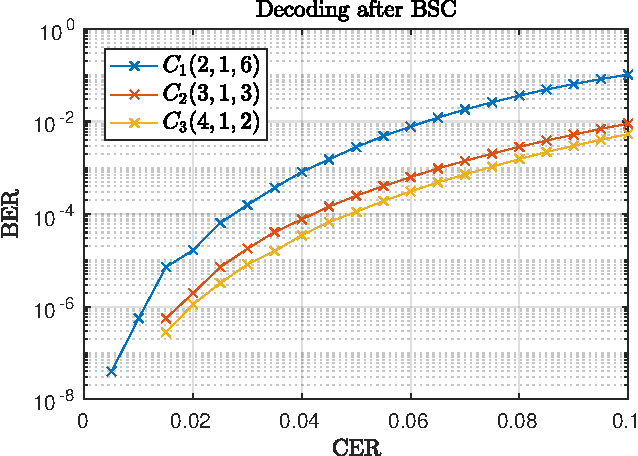
\includegraphics[scale=1]{../figures/qirandom.pdf} 
\caption{Given codes\todo[inline]{change caption}\label{fig:givenRandomFigure}}
\end{figure}

\begin{figure}
\centering
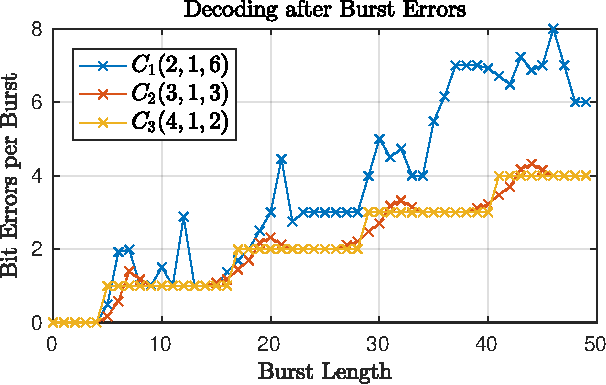
\includegraphics[scale=1]{../figures/qiburst.pdf} 
\caption{Given Codes\todo[inline]{change caption}\label{fig:givenBurstFigure}}
\end{figure}

\begin{figure}
\centering
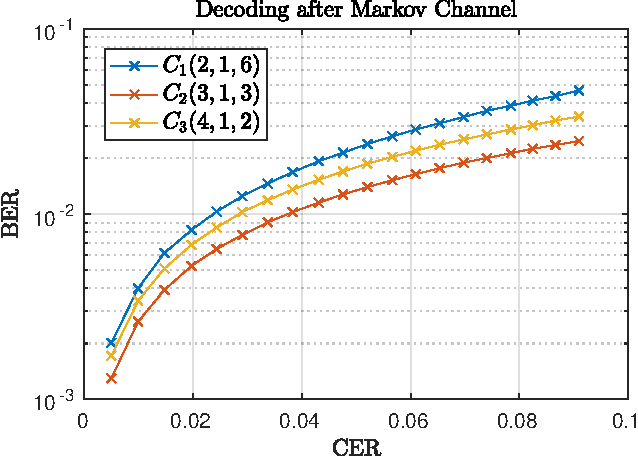
\includegraphics[scale=1]{../figures/qimarkov.pdf} 
\caption{Given Codes.\todo[inline]{change caption}\label{fig:givenMarkovFigure}}
\end{figure}
